\chapter{Comment mettre à jour le firmware de votre ToM+}
\label{sec:update_procedure}

\section{Prérequis avant la mise à jour}

ToM+ évolue constamment, car presque chaque jour je reçois des suggestions pour améliorer
certaines fonctionnalités ou même en ajouter de très intéressantes. J'essaie de prendre en compte tous les
conseils de chaque propriétaire, et ces conseils et idées se traduisent par des mises à jour du firmware.
Lors des tests de l'appareil en conduite, si vous remarquez des bugs ou des comportements étranges, n'hésitez pas à me les
signaler afin qu'ils fassent l'objet de correctifs. Comme je l'ai dit au début,
ToM+ s'améliore continuellement, alors restez à l'écoute\ldots

\subsection{Pourquoi devrais-je mettre à jour ?}

Une nouvelle mise à jour apporte de nouvelles fonctionnalités et des corrections de bugs, alors pourquoi conserver une ancienne
version du firmware quand vous pouvez facilement installer la dernière version stable ? Il n'y a donc aucune
raison de garder votre ToM+ obsolète, puisque la mise à jour de son logiciel est \textbf{gratuite à vie}
et vous procurera beaucoup de satisfaction et de plaisir en essayant les nouvelles fonctionnalités. En fin de compte, je vous conseille
personnellement de maintenir votre ToM+ à jour pour plus de sécurité.\\

Quoi qu'il en soit, toutes les anciennes versions du firmware restent disponibles sur le forum Twizy dans la section ToM
(\url{https://www.twizy-forum.de/twiz-o-meter}) sous les sujets \textit{“[Twiz o'meter] Update to
firmware x.x”}. En fait, ToM+ permet également les retours à une version antérieure (downgrades) si nécessaire.

\subsection{De quoi ai-je besoin pour la mise à jour ?}

Dans les sections suivantes, nous aborderons une méthode alternative de mise à jour, nettement plus
chronophage par rapport à la méthode OTA déjà expliquée dans la Section~\ref{sec:web_ota_update}.
Je \textbf{recommande personnellement la méthode OTA}, car elle est plus sûre et plus facile à réaliser si vous n'êtes pas
vraiment expert en informatique et systèmes embarqués.\\

Si vous êtes toujours convaincu de vouloir mettre à jour le firmware de votre ToM+ avec la seconde méthode, il y a
quelques éléments dont vous aurez besoin pour mener à bien la mise à jour. Tout
d'abord, il vous faudra un ordinateur (un ordinateur de bureau ou un portable fera parfaitement l'affaire).

Plus tard, nous verrons comment connecter ToM+ à notre ordinateur afin de lui transférer les nouveaux
fichiers de mise à jour. La deuxième chose à vous procurer est un câble micro-USB, le même
que celui habituellement utilisé pour les appareils rechargeables et les anciens smartphones. Vous aurez
également besoin d'une carte microSD d'une capacité de stockage comprise entre 8 et 32 Go.~Des exemples
sont présentés sur les photos ci-dessous. Et bien sûr, vous aurez besoin de votre ToM+ !

\begin{figure}[H]
    \centering
    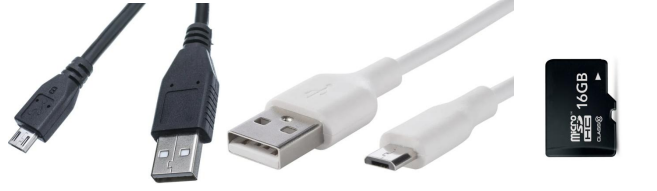
\includegraphics[width=0.8\textwidth]{figures/cables_sd_update.png}
    \caption{Câbles microUSB et exemple de carte microSD.}
\end{figure}


\subsection{À quoi ressemblent les fichiers de mise à jour ?}
\label{sec:update_files}

Avant de mettre à jour le firmware, vous devez évidemment télécharger depuis le forum Twizy
(à nouveau \url{https://www.twizy-forum.de/twiz-o-meter}) le fichier ZIP de la version souhaitée.~Vous
devrez probablement vous inscrire sur le forum pour voir et télécharger les fichiers de firmware et
les images. C'est une communauté très sympathique et active, je vous conseille donc de devenir membre quoi qu'il en soit.
Après avoir extrait les fichiers dans le dossier, voici ce que vous devriez obtenir :

\begin{figure}[H]
    \centering
    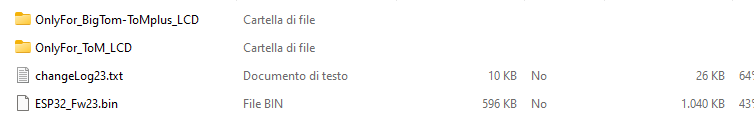
\includegraphics[width=1\textwidth]{figures/firmware_release_folder.png}
    \caption{Liste des fichiers du dossier de version du firmware.}
\end{figure}

Tout d'abord, nous remarquons un fichier texte nommé \textit{changeLog23.txt}, utilisé pour suivre
les fonctionnalités ajoutées et les bugs corrigés dans la dernière version du firmware. Lisez-le si vous êtes
curieux de savoir ce qui est nouveau ou si vous avez besoin d'aide supplémentaire pour la procédure de mise à jour.\\

Ensuite, il y a deux dossiers contenant la mise à jour du \textbf{firmware de l'écran LCD} au format \textit{.tft}.
\textbf{Choisissez la version} conçue pour votre appareil : le premier dossier si vous possédez un ToM+ ou un
BigToM (c'est-à-dire avec un plus grand écran), ou l'autre si vous avez un ToM traditionnel ou si
vous souhaitez mettre à jour le Twin ToM (écran plus petit). C'est une étape
cruciale, sinon les nouvelles icônes et graphismes ne s'adapteront pas à la taille de votre écran.\\

Le dernier fichier est le fichier binaire \textit{ESP32\textunderscore Fw23.bin} pour la \textbf{mise à jour du boîtier noir}.
Assurez-vous de posséder tous ces fichiers, car vous en aurez besoin dans les étapes suivantes.

\subsection{Que dois-je savoir avant la mise à jour ?}

Préparons maintenant notre ToM+ pour la mise à jour en \textbf{basculant l'interrupteur sur OFF} sur le
boîtier noir. Assurez-vous de l'éteindre (\textit{c'est-à-dire le symbole 0 sur l'interrupteur}), sinon
vous causerez très certainement de graves problèmes au ToM+.

Ainsi, si votre Twizy est toujours sous tension avec la clé sur le contact, éteignez-la complètement
et retirez la clé de contact. Après ces étapes simples, vous êtes prêt à commencer la procédure
de mise à jour, mais veillez à suivre scrupuleusement les instructions de ce guide. Ne
procédez pas par intuition, sous peine de risquer de bloquer définitivement (bricker) votre appareil.\\

Le processus de mise à jour est assez simple et vous devrez mettre à jour à la fois le firmware de l'écran LCD
et celui du boîtier noir, dans cet ordre précis. Nous verrons comment procéder dans la section suivante.



\section{Mise à jour du firmware de l'écran LCD}

L'écran LCD est l'un des composants essentiels de ToM+, comme cela a été abordé dans les deux
premiers chapitres, et pour cette raison, il doit également être mis à jour. Un nouveau firmware
signifie de nouvelles icônes et des dispositions différentes, et pour pouvoir les charger sur l'écran,
il est crucial d'utiliser une petite \textbf{carte microSD}. L'emplacement
pour carte SD du ToM+ se trouve sous l'écran ; vous devrez donc peut-être le retirer temporairement de votre
boîte à gants pour pouvoir y travailler plus facilement, ou simplement le basculer vers l'arrière et
vous verrez l'ouverture.

\subsection{Préparation de la carte microSD}

Malheureusement, toutes les cartes microSD ne fonctionnent pas avec l'écran, en particulier les plus récentes
conçues pour les appareils photo, mais pour l'instant, j'ai testé des cartes Classe 10 HC de 8 à 32 Go et elles
semblent bien fonctionner. N'hésitez pas à essayer avec votre propre carte mémoire pour voir si elle fonctionne.\\

Maintenant que nous avons choisi une carte microSD, qui doit avoir une capacité de stockage \textbf{comprise entre 8
et 32 Go}, nous devons y copier le firmware LCD. Avant de copier le fichier sur la carte,
nous devons nous assurer qu'il n'y a pas d'autres fichiers, sinon la mise à jour ne fonctionnera pas.

Déplacez donc tous vos fichiers vers votre ordinateur et formatez la carte microSD au \textbf{format FAT32}
comme je l'ai fait sur la capture d'écran ci-contre. Pour ce faire, faites un clic droit sur l'icône de la carte dans votre
explorateur de fichiers et sélectionnez l'option \textbf{“Formater”} dans le menu déroulant.

\begin{figure}[H]
    \centering
    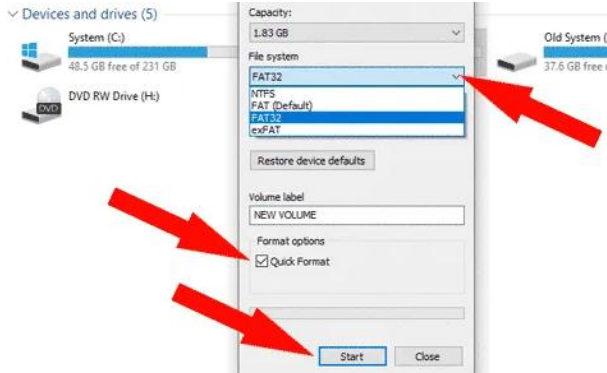
\includegraphics[width=0.7\textwidth]{figures/forma_sd_steps.png}
    \caption{Étapes pour formater la microSD en FAT32.}
\end{figure}

Comme montré sur l'image, sélectionnez le système de fichiers \textbf{FAT32}, puis cochez l'option
\textbf{“Formatage rapide”} et appuyez sur le bouton \textbf{“Démarrer”} pour lancer le
processus. Patientez jusqu'à la fin, puis copiez le fichier \textit{.tft} fourni dans
la version du firmware que vous souhaitez installer, situé dans le dossier ZIP de mise à jour.


\subsection{Insertion de la carte microSD}

Nous sommes maintenant prêts à insérer la carte microSD dans l'emplacement de l'écran LCD. Il peut être utile
d'utiliser une pince à bec fin pour insérer délicatement la carte microSD. Cela vous permettra
de bien centrer la carte dans l'emplacement interne.\\

\textbf{RAPPEL !} La carte microSD ne s'insère dans l'emplacement que dans un seul sens, le côté des contacts
orienté vers la surface de l'écran, comme montré sur l'image. Si elle ne rentre pas, ne forcez pas !
Essayez de la tourner de l'autre côté.

Maintenant que la carte microSD est insérée dans l'emplacement interne, poussez-la doucement dans le
boîtier jusqu'à entendre un « clic ». Cela signifie que vous pouvez retirer la pince
en toute sécurité sans risquer de perdre la carte à l'intérieur du boîtier.

\begin{figure}[H]
    \centering
    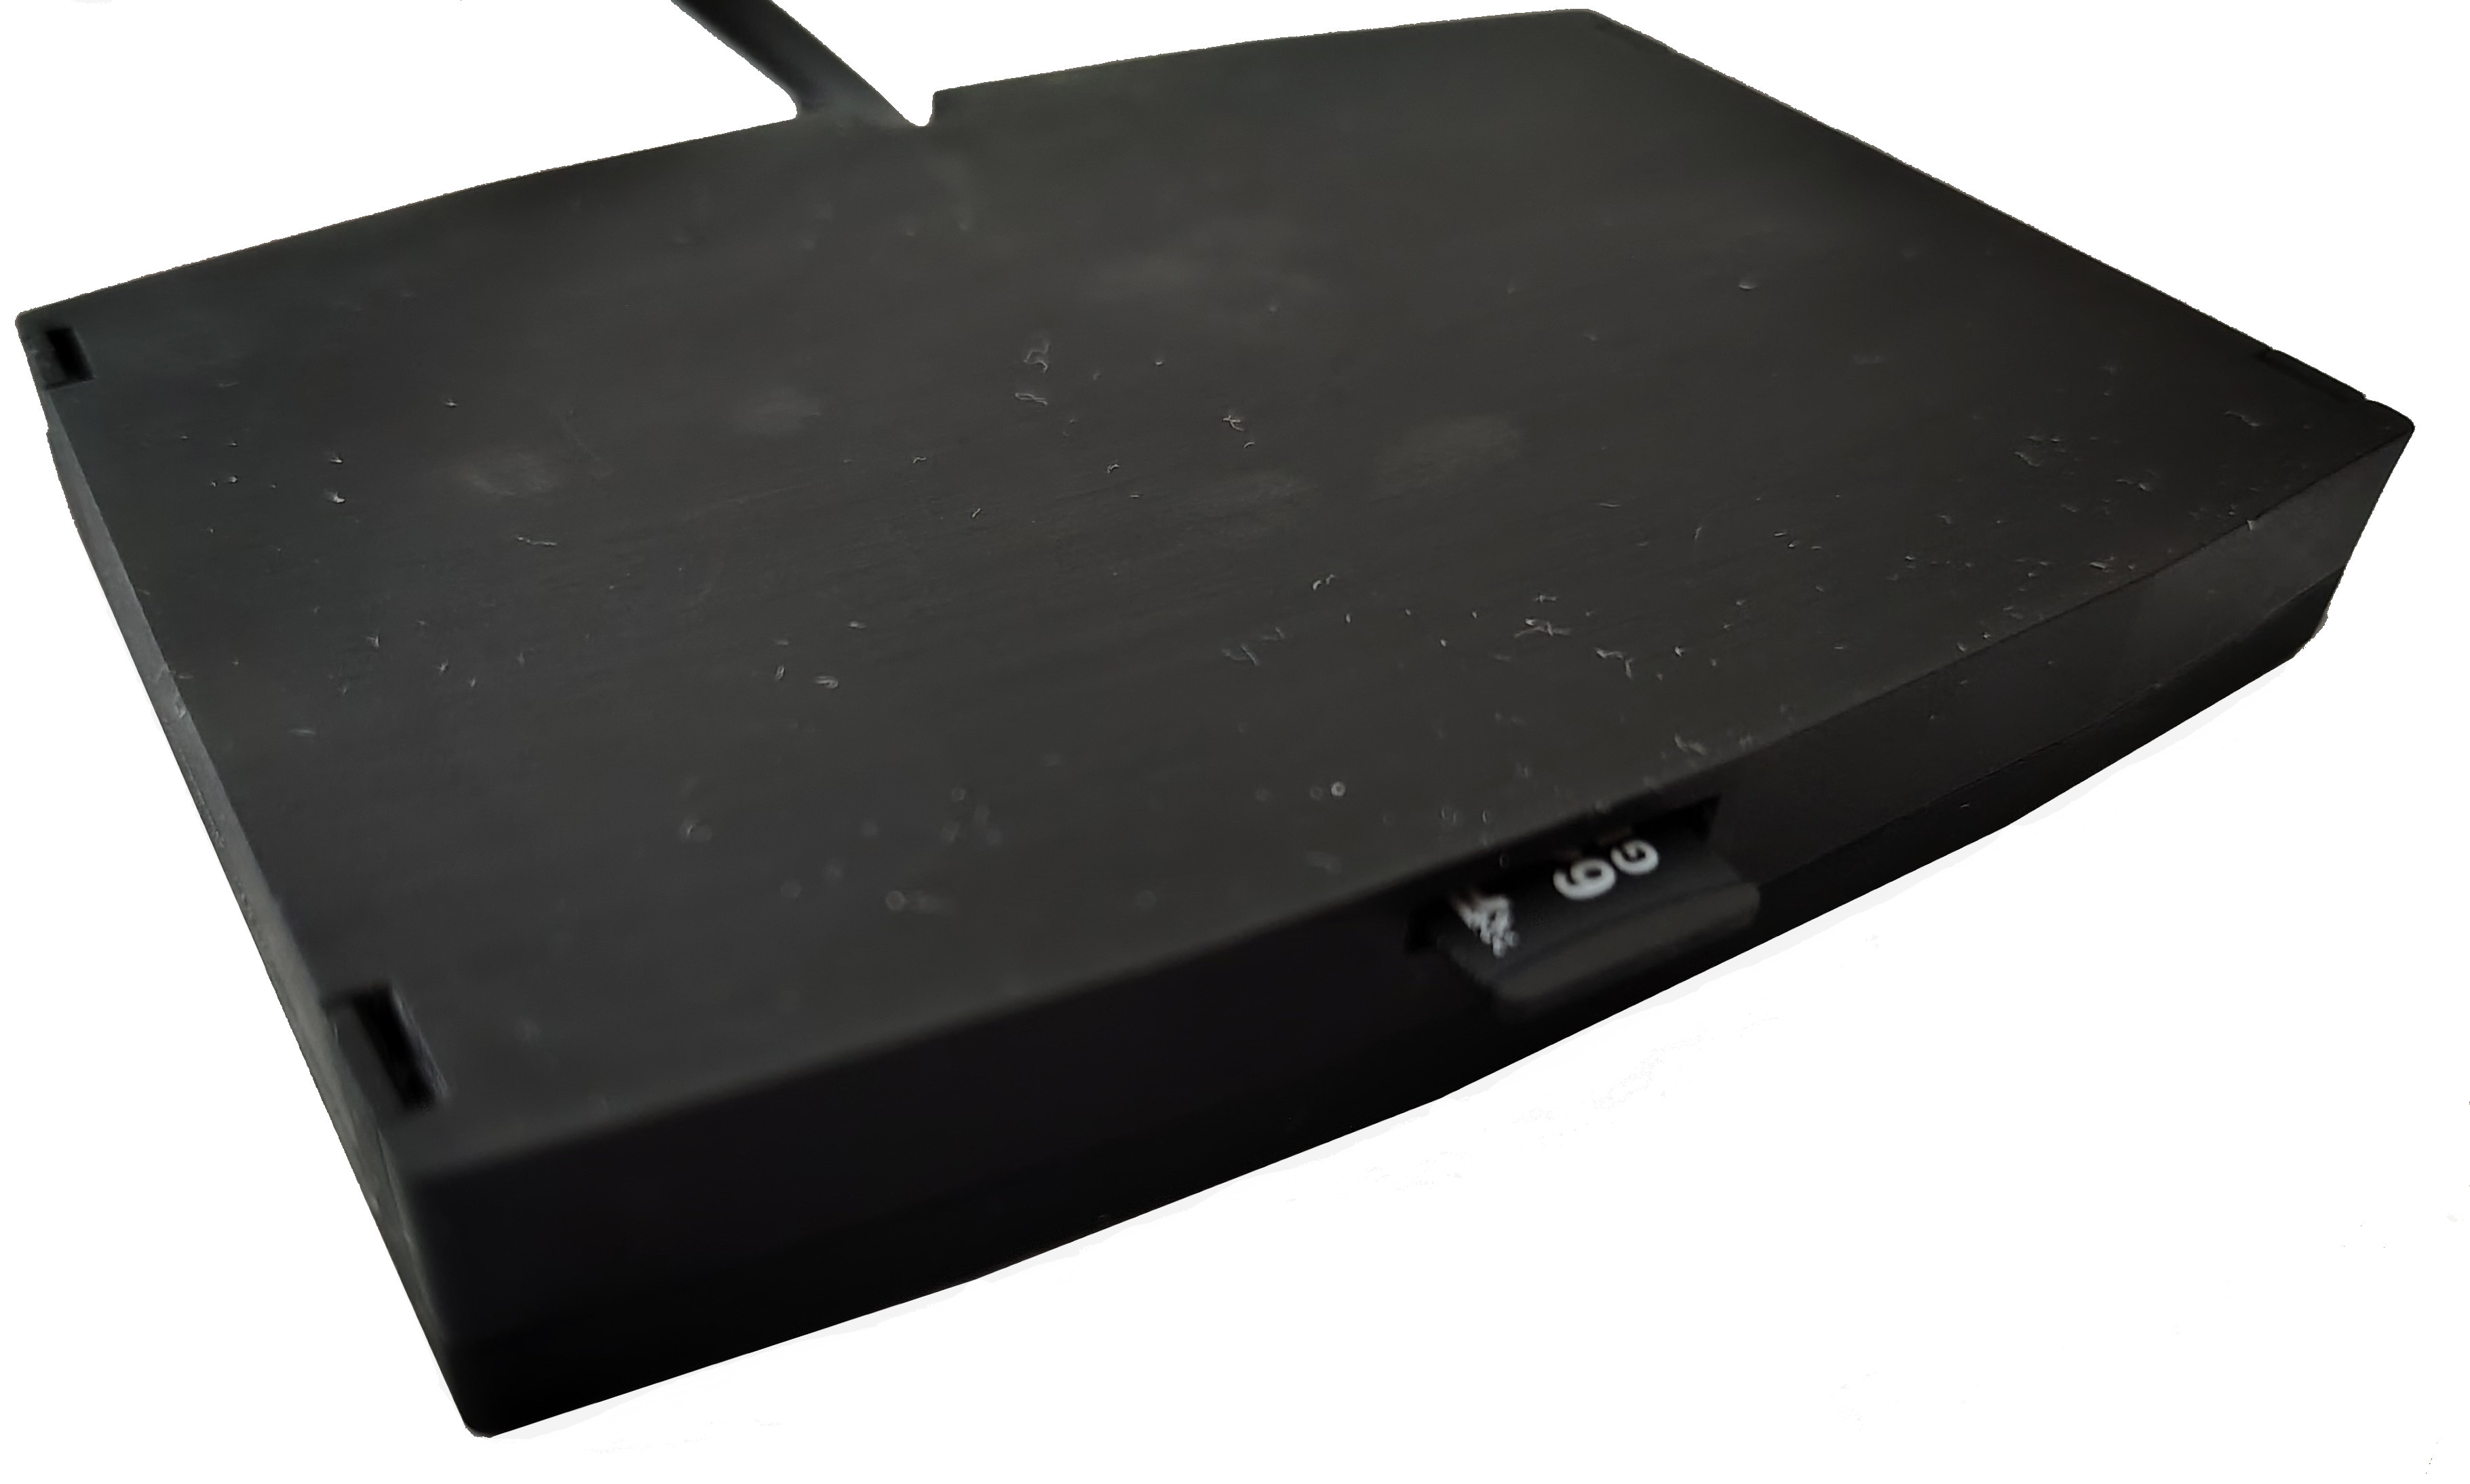
\includegraphics[width=0.6\textwidth]{figures/sd_insert.jpg}
    \caption{Insérer la microSD dans l'ouverture de l'écran.}
\end{figure}


\subsection{Déroulement de la mise à jour}

Une fois la microSD insérée, nous pouvons poursuivre la procédure de mise à jour. Retournez à
votre Twizy et rebranchez l'écran au boîtier noir. Ensuite, allumez
l'écran à l'aide de l'interrupteur du boîtier noir (\textit{c'est-à-dire le symbole 1 sur l'interrupteur}), et
seulement après cela, mettez le contact de votre Twizy avec la clé.

Attendez que l'écran LCD lance le processus de mise à jour jusqu'à ce que vous voyiez le pourcentage
de progression s'afficher, comme le montre la figure ci-dessous (pour l'écran du ToM+ comme du ToM).
Le processus de copie depuis la microSD prend généralement jusqu'à une minute et demie.

\begin{figure}[ht]
    \centering

    \begin{subfigure}[t]{0.48\textwidth}
        \centering
        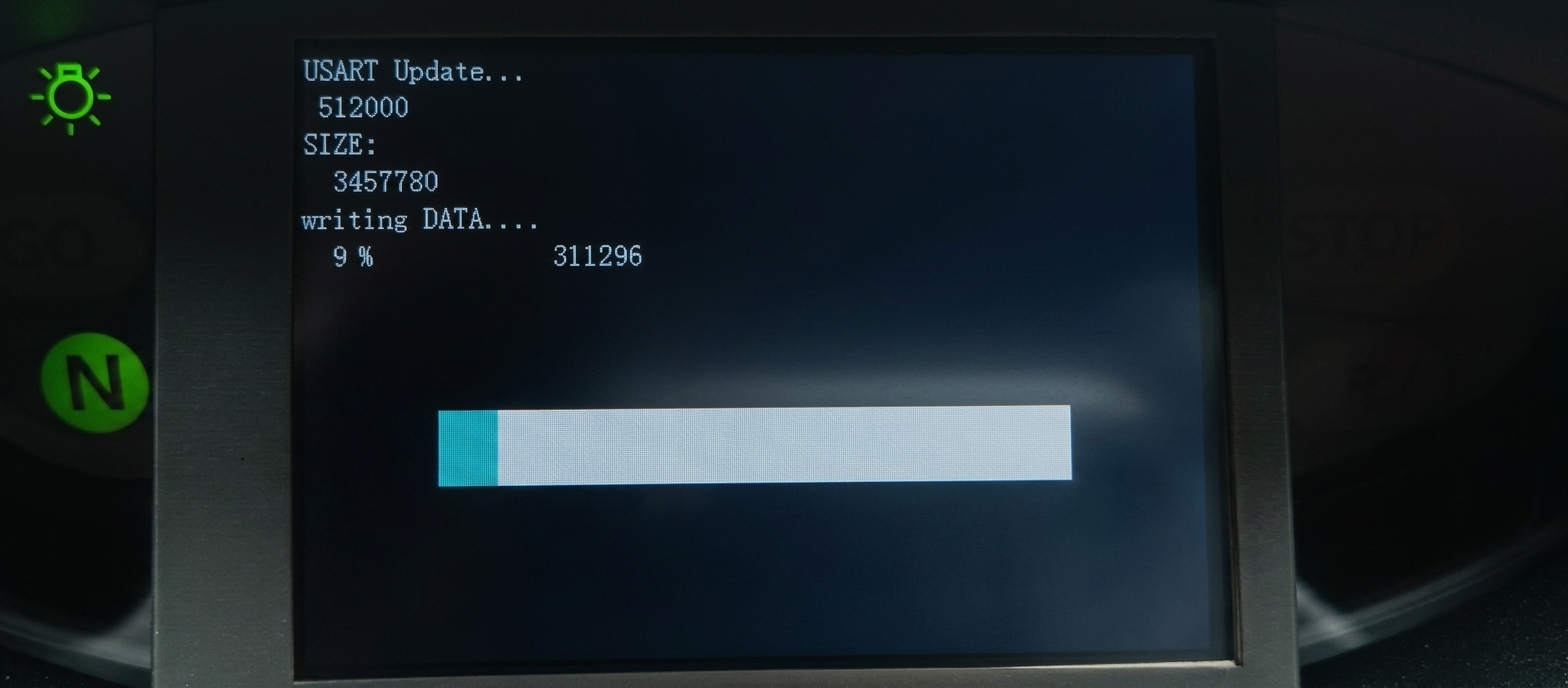
\includegraphics[width=\linewidth]{figures/update_screen_lcd.jpg}
        \caption{Mise à jour de l'écran du ToM+.}
    \end{subfigure}
    \hfill
    \begin{subfigure}[t]{0.48\textwidth}
        \centering
        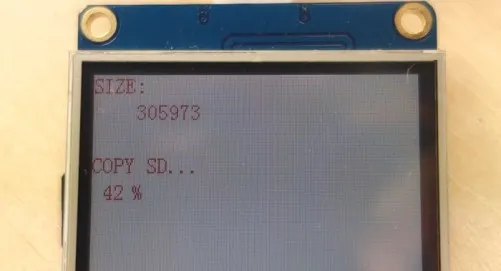
\includegraphics[width=\linewidth]{figures/copy_sd_card.png}
        \caption{Mise à jour de l'écran du ToM.}
    \end{subfigure}
\end{figure}

Une fois la mise à jour du firmware LCD terminée avec succès, cet écran s'affichera,
indiquant \textbf{“Update Succeeded!”} (Mise à jour réussie !). Après la mise à jour, \textbf{NE PAS}
rallumer l'appareil avec la carte microSD insérée ! Nous pouvons maintenant éteindre le véhicule et éteindre
à nouveau ToM+ via l'interrupteur du boîtier noir.

Ensuite, retirez la carte microSD pendant que l'ensemble du système est hors tension ; la mise à jour
de l'écran LCD est terminée. \textbf{RAPPEL !} Si vous retirez la carte alors que ToM+ est sous tension,
vous bloquerez définitivement (bricker) l'appareil ! Après cela, sans modifier l'état général du
système, passons à la mise à jour du boîtier noir, comme expliqué dans la section suivante.



\section{Mise à jour du firmware du boîtier noir (Windows)}

Le boîtier noir est le deuxième composant essentiel du ToM+ et constitue le cerveau de tout
le système. Si nous mettons à jour uniquement l'écran, le boîtier noir ne saura pas à quoi
correspondent ces nouvelles icônes, ce qui entraînera des erreurs de communication.

Il est donc crucial d'installer également le nouveau firmware sur la carte mère du ToM+. Pour ce
faire, nous n'aurons plus besoin de la carte microSD, mais nous utiliserons le câble microUSB
préparé précédemment et l'ordinateur. En effet, nous allons flasher le firmware directement sur
la carte ESP32 pour y installer le nouveau logiciel.


\subsection{Préparation de l'ordinateur}

Avant de brancher le câble sur l'ordinateur, nous devons installer certains programmes pour qu'il
fonctionne correctement. La \textbf{carte ESP32} nécessite des pilotes (drivers) pour être reconnue par le
système d'exploitation ; nous allons donc les télécharger directement depuis le site officiel.

Depuis la page de téléchargement du \href{https://www.silabs.com/software-and-tools/usb-to-uart-bridge-vcp-drivers?tab=downloads}{site Silicon Labs},
nous devons choisir la version correspondant à notre système d'exploitation, comme le montre la capture d'écran ci-dessous.

\begin{figure}[H]
    \centering
    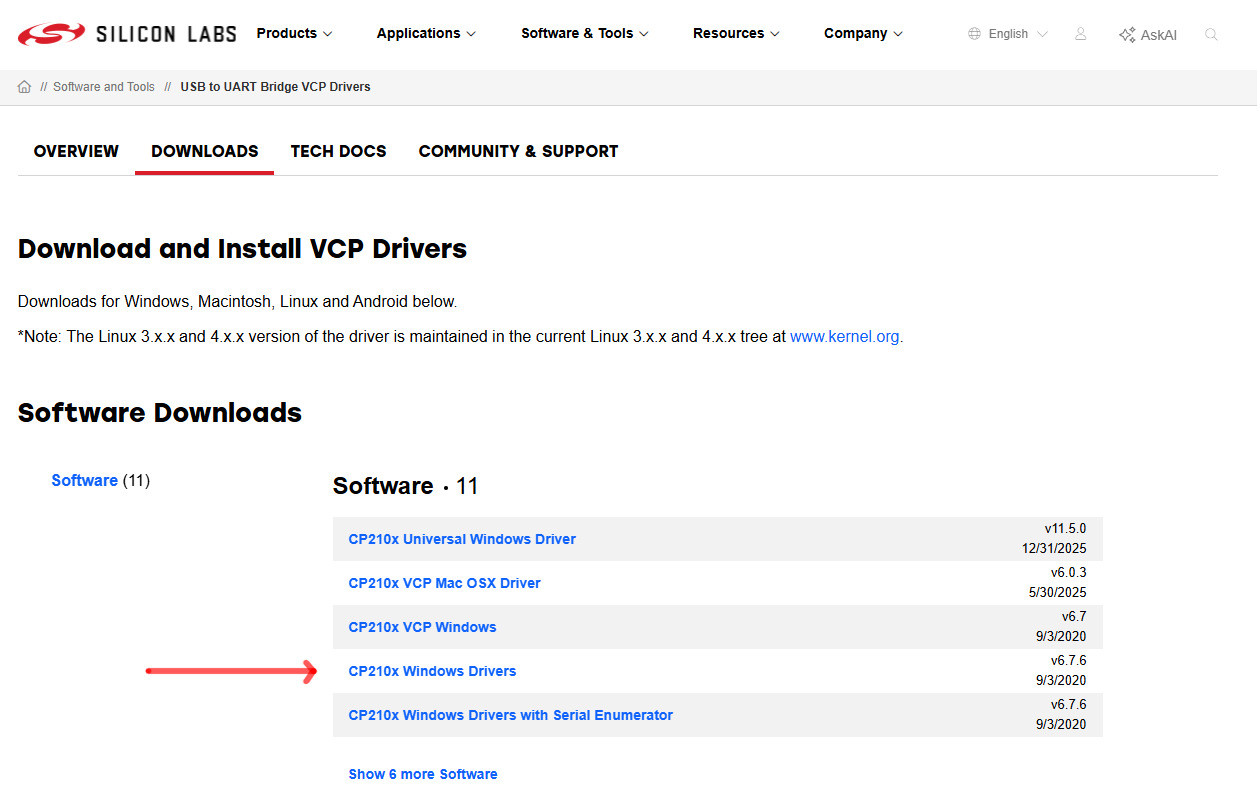
\includegraphics[width=1\textwidth]{figures/driver_download.png}
    \caption{Page de téléchargement des pilotes sur Silicon Labs.}
\end{figure}

Cette section du guide étant spécifique au système d'exploitation Windows, nous allons
télécharger le paquet \textit{“CP210x Windows Drivers”} en cliquant sur le lien surligné
en jaune sur l'image ci-dessus.

Le fichier téléchargé sera une archive ZIP, généralement nommée \textit{“CP210x\textunderscore Windows\textunderscore Drivers.zip”},
contenant quelques dossiers et plusieurs fichiers. La capture d'écran ci-dessous présente
la liste habituelle des fichiers contenus dans l'archive ZIP.

\begin{figure}[H]
    \centering
    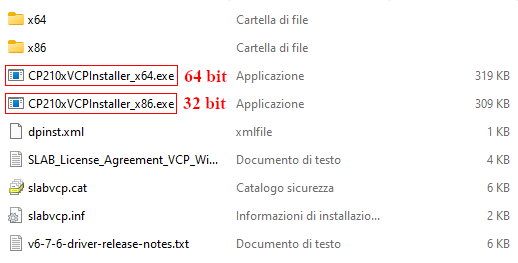
\includegraphics[width=0.7\textwidth]{figures/driver_folder.png}
    \caption{Contenu de l'archive ZIP des pilotes.}
\end{figure}

Extrayez tous les fichiers dans un dossier temporaire sur votre Bureau. Il est maintenant important de
choisir le bon fichier \textit{“.exe”} à exécuter pour installer les pilotes. Si votre
système d'exploitation est en 64 bits (ce qui est le cas de la plupart des ordinateurs), exécutez le fichier \textit{CP210xVCPInstaller\textunderscore x64.exe} ;
sinon, le second fichier \textit{“.exe”} sera celui adapté, comme le montre l'image.

Veillez à exécuter le fichier exécutable avec les privilèges d'administrateur en faisant un clic droit dessus et en
sélectionnant l'option \textbf{“Exécuter en tant qu'administrateur”}. Si vous y êtes invité, autorisez le programme à effectuer
des opérations d'administration sur votre ordinateur, faute de quoi le processus d'installation du pilote ne démarrera pas.

\begin{figure}[ht]
    \centering

    \begin{subfigure}[t]{0.48\textwidth}
        \centering
        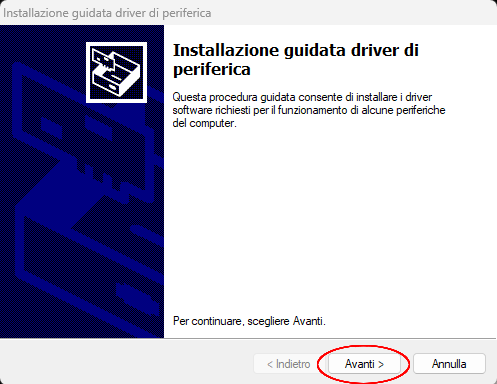
\includegraphics[width=\linewidth]{figures/wizard_step1.png}
        \caption{Première étape : Appuyez sur « Suivant ».}
    \end{subfigure}
    \hfill
    \begin{subfigure}[t]{0.48\textwidth}
        \centering
        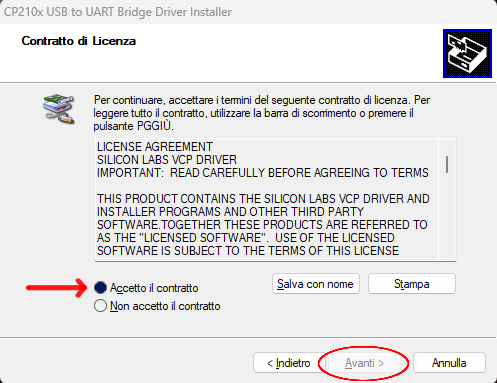
\includegraphics[width=\linewidth]{figures/wizard_step2.png}
        \caption{Deuxième étape : « Accepter » puis « Suivant ».}
    \end{subfigure}
\end{figure}

Une fois l'assistant d'installation lancé, une fenêtre semblable à celle de gauche s'affiche. Il s'agit d'un
outil d'installation pas à pas pour les pilotes nécessaires à la reconnaissance du boîtier noir par votre
ordinateur. Appuyez sur le bouton \textbf{“Suivant”} comme indiqué ici pour démarrer le processus.\\

La fenêtre suivante qui devrait apparaître est celle présentée à droite. Ici,
vous devez accepter la licence en cochant la première option \textbf{“Accepter la licence”}. Ensuite,
vous pouvez cliquer sur le bouton \textbf{“Suivant”} comme indiqué et démarrer la copie des pilotes
dans le bon dossier système : patientez jusqu'à la fin de la copie.

Une fois la copie terminée, l'installation des pilotes CP210X est achevée et vous pouvez
brancher le boîtier noir à votre ordinateur en toute sécurité. Cliquez ensuite sur le bouton \textbf{“Terminer”}
pour fermer la fenêtre.\\

Avant de faire quoi que ce soit, assurez-vous que l'interrupteur du boîtier noir ToM+ est bien
éteint (\textit{c'est-à-dire le symbole 0 sur l'interrupteur}). La Twizy doit également être hors tension,
car si vous branchez le câble sur votre PC alors que le ToM+ est encore alimenté par le
véhicule, vous allez mélanger les alimentations (5V et 12V) et le ToM+ sera définitivement endommagé.

\begin{figure}[H]
    \centering
    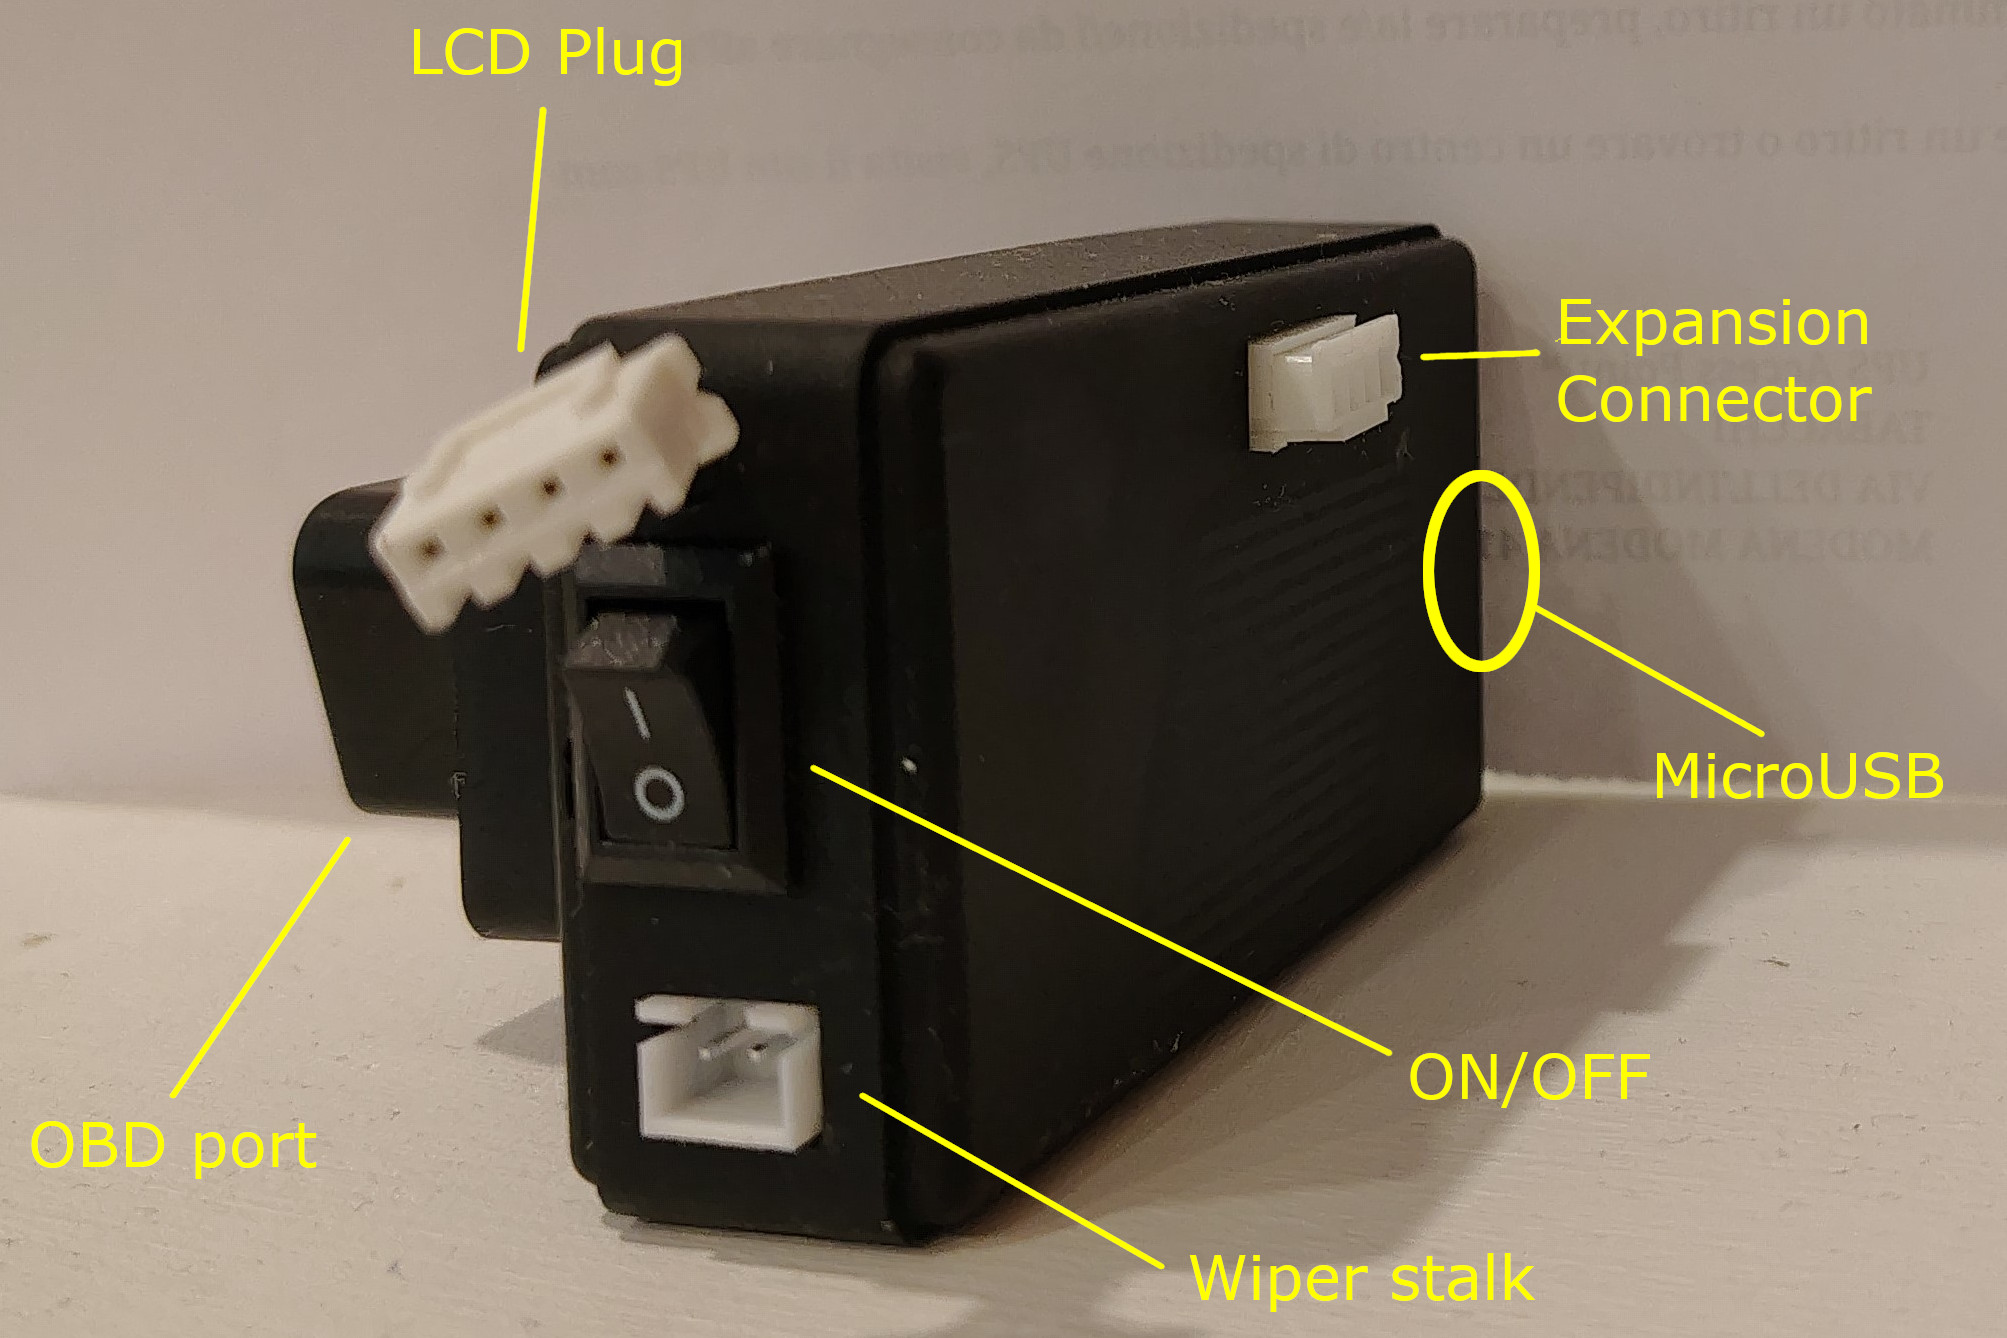
\includegraphics[width=0.6\textwidth]{figures/black_box.jpg}
    \caption{Les composants du boîtier noir.}\label{fig:black_box_labels}
\end{figure}

Le boîtier noir dispose d'un petit connecteur microUSB sur sa face arrière, comme
vous pouvez le voir sur l'image ci-dessus. Connectez donc l'extrémité microUSB du câble au boîtier noir.
Ensuite, connectez l'extrémité USB du câble à un port USB libre de votre ordinateur.

\textbf{RAPPEL !} Les deux extrémités du câble ne s'insèrent que dans un seul sens dans les prises correspondantes,
ne forcez donc pas au risque d'endommager le port du ToM+ ou celui de votre ordinateur.
Essayez de le tourner de l'autre côté et vérifiez si cela fonctionne ainsi.\\

Désormais, l'ordinateur devrait reconnaître la carte ESP32 du boîtier noir si vous avez correctement installé les
pilotes. Pour le vérifier, recherchez l'application \textbf{“Gestionnaire de périphériques”}
sur votre PC et exécutez-la.

Une fenêtre similaire à celle de la figure ci-dessous devrait s'ouvrir.
Recherchez la ligne \textbf{“Ports (COM et LPT)”} avec une icône de connecteur et double-cliquez dessus pour ouvrir
la liste de tous vos périphériques série. Comme sur la capture d'écran, recherchez \textit{“Silicon Labs
CP210x to UART Bridge (COMx)”} puis notez le numéro du port COM, qui est
\textbf{COM8} dans cet exemple. Ce numéro sera utile à l'étape suivante pour indiquer au PC
où télécharger la nouvelle version du firmware. Poursuivons le processus\ldots

\begin{figure}[H]
    \centering
    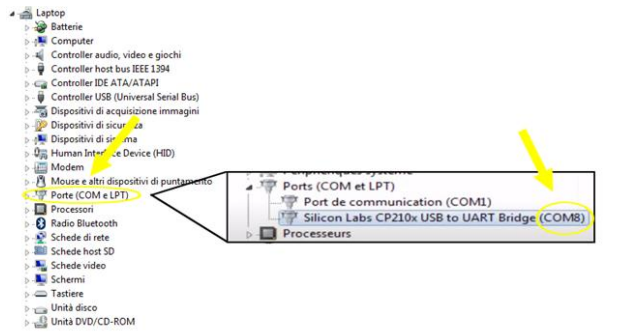
\includegraphics[width=0.8\textwidth]{figures/device_manager.png}
    \caption{Gestionnaire de périphériques - Port série UART (COM8).}
\end{figure}

Visitez le \href{https://www.espressif.com/en/support/download/other-tools}{site officiel d'ESP32}
pour télécharger un outil nécessaire pour flasher le firmware sur la carte du boîtier noir.
Recherchez \textbf{“Flash Download Tools”} et cliquez sur le bouton comme indiqué sur l'image.
Ensuite, recherchez dans la page les \textit{“Flash Download Tools”} avec l'icône de disquette et cliquez dessus.

Un fichier ZIP nommé \textit{“flash\textunderscore download\textunderscore tool\textunderscore x.x.x.zip”} sera téléchargé,
où les symboles « x » seront remplacés par le nom de la version, qui est \textbf{V3.9.11} dans cet exemple.
En ouvrant le dossier ZIP téléchargé, vous remarquerez qu'il contient un autre dossier.
Extrayez-le sur votre Bureau ou à l'emplacement de votre choix, puis ouvrez-le. Les fichiers
qu'il contient sont généralement ceux énumérés sur la capture d'écran ci-dessous.

\begin{figure}[H]
    \centering
    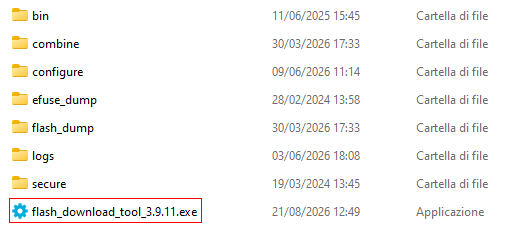
\includegraphics[width=0.7\textwidth]{figures/esptool_folder.png}
    \caption{Contenu du dossier ZIP des Flash Tools.}
\end{figure}

Sélectionnez \textit{“flash\textunderscore download\textunderscore tool\textunderscore 3.9.11.exe”}
ou la version que vous avez téléchargée et exécutez-le avec les droits d'administrateur en faisant un clic droit
sur le fichier et en choisissant l'option \textbf{“Exécuter en tant qu'administrateur”}.
Si vous y êtes invité, autorisez l'exécutable à effectuer des opérations sur votre ordinateur.\\

Une fois le programme lancé, une fenêtre de terminal s'ouvre, qui va lancer
en quelques secondes l'interface utilisateur. Elle devrait ressembler à la première image
présentée dans l'exemple ci-dessous. Vous devez modifier le champ \textbf{“ChipType”} pour choisir \textit{“ESP32”},
comme indiqué dans la deuxième étape ci-dessous. Laissez le reste inchangé et appuyez sur le bouton \textbf{“OK”}.

\begin{figure}[H]
    \centering
    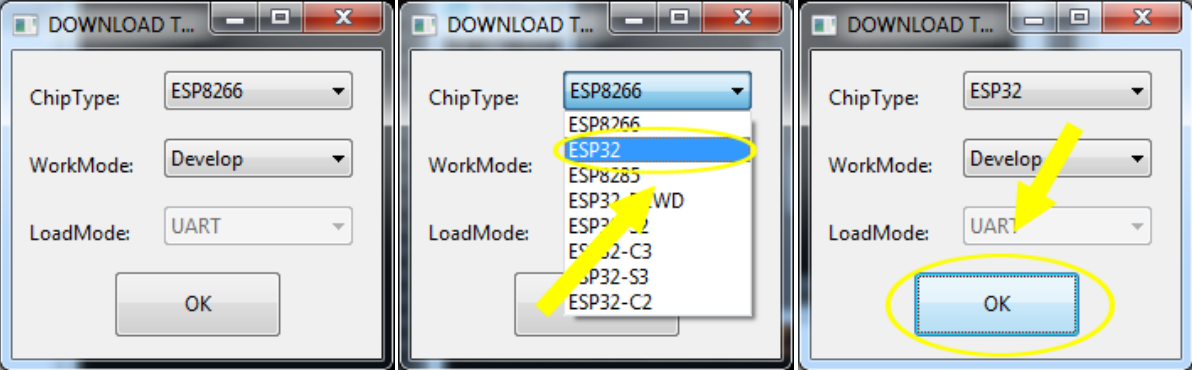
\includegraphics[width=0.85\textwidth]{figures/launching_flashtool.png}
    \caption{Sélection de la carte mère ESP32 dans le menu de choix.}
\end{figure}


\subsection{Déroulement de la mise à jour}

Dès que vous appuyez sur le bouton \textbf{“OK”}, la fenêtre \textit{“ESP32 DOWNLOAD TOOL”} s'ouvre.
Extrayez maintenant le fichier binaire (extension \textit{.bin}) fourni dans le fichier ZIP de publication du
firmware ToM+, comme nous l'avons vu à la Section~\ref{sec:update_files}.

Ensuite, appuyez sur le bouton \textbf{“\ldots”} visible sur la première image et sélectionnez le chemin d'accès du fichier \textit{“.bin”}.
Une fois cette opération effectuée, appuyez sur le bouton \textbf{“Ouvrir”} : une ligne verte contenant
le chemin que vous venez de valider apparaît sur la première ligne.

Poursuivez en \textbf{cochant la case} située à côté de la première ligne, désignant le firmware que vous
souhaitez charger. Saisissez ensuite dans la zone de texte visible sur la deuxième image la séquence
de caractères suivante : \textbf{0$\times$10000} (avec quatre zéros). Cela représente l'adresse mémoire initiale
où seront stockés les fichiers du firmware.

Vient enfin la dernière étape de la configuration : sélectionnez le numéro de port COM
dans la liste déroulante située dans le coin inférieur droit. Veillez à sélectionner le bon port COM,
c'est-à-dire celui que nous avons précédemment noté depuis le \textbf{Gestionnaire de périphériques}.

\begin{figure}[H]
    \centering
    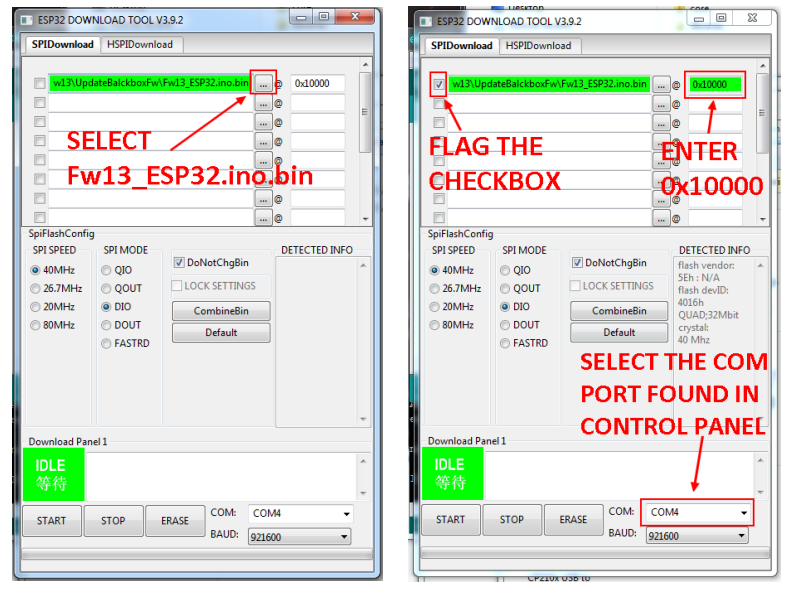
\includegraphics[width=1\textwidth]{figures/flashtool_page.png}
    \caption{Étapes de configuration de l'outil ESP32 Download Tool.}
\end{figure}

Lançons à présent la mise à jour en appuyant sur le bouton \textbf{“START”} comme indiqué sur la première image.
Une barre de progression verte apparaît en bas de la fenêtre et l'ensemble du processus
prend généralement deux minutes.

Une fois le transfert terminé, le message \textbf{“FINISH”} s'affiche dans le cadran vert
dans le coin inférieur gauche, comme montré sur l'image.
En guise de confirmation supplémentaire, la barre de progression sera complète : la mise à jour est désormais terminée.

\begin{figure}[H]
    \centering
    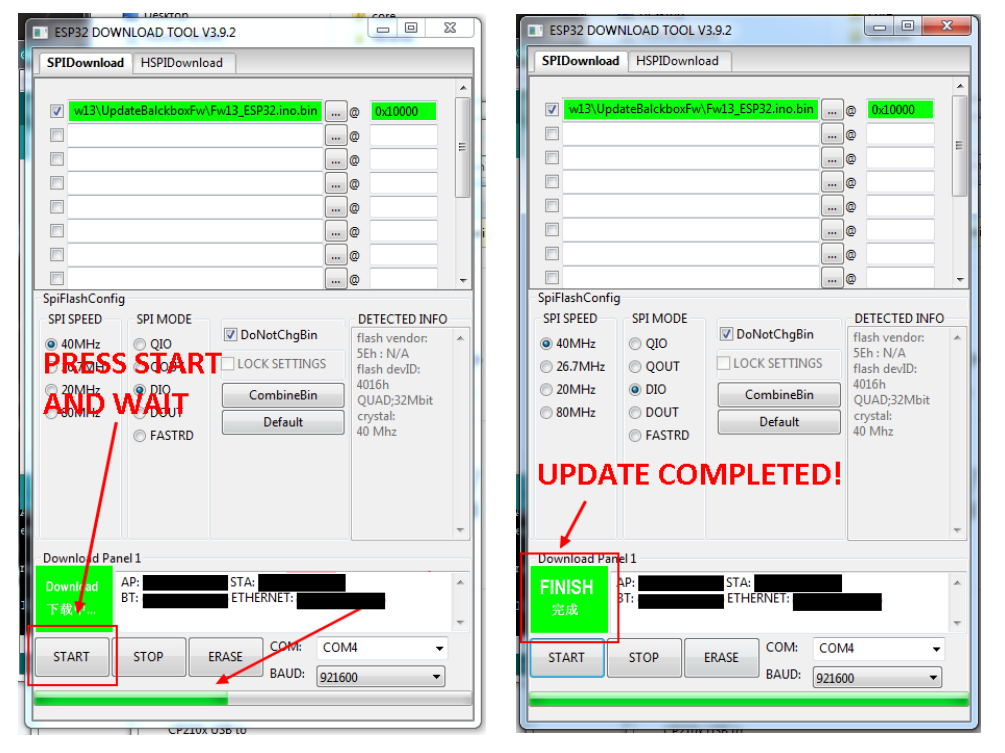
\includegraphics[width=1\textwidth]{figures/flashtool_page2.png}
    \caption{Finalisation de la mise à jour dans ESP32 Download Tool.}
\end{figure}

Fermez cette fenêtre, puis vous pouvez débrancher le câble en toute sécurité, côté PC
et côté ToM+. Ce n'est qu'après ces actions que vous pourrez rétablir l'alimentation normale du ToM+,
en basculant l'interrupteur sur la position 1 et en mettant le contact de votre Twizy avec la clé.

Pour restaurer vos configurations précédentes, accédez à la page des paramètres du ToM+ en appuyant sur
les trois points dans le coin supérieur droit, puis appuyez sur le bouton de sortie sans rien
modifier. De cette façon, vous mettrez à jour la structure des données enregistrées dans la mémoire
du boîtier noir et vos configurations seront à nouveau opérationnelles.\\

\textbf{Félicitations !} Vous avez terminé l'ensemble de la procédure de mise à jour. Profitez bien du nouveau firmware,
et n'oubliez pas de me signaler tout bug ou problème par message privé, idéalement en joignant une photo.

\clearpage

\section{Mise à jour du boîtier noir (Unix)}

Le boîtier noir est le deuxième composant essentiel du ToM+ et constitue le cerveau de tout
le système. Si nous mettons à jour uniquement l'écran, le boîtier noir ne saura pas à quoi
correspondent ces nouvelles icônes, ce qui entraînera des erreurs de communication.

Il est donc crucial d'installer également le nouveau firmware sur la carte mère du ToM+. Pour ce
faire, nous n'aurons plus besoin de la carte microSD, mais nous utiliserons le câble microUSB
préparé précédemment et l'ordinateur. En effet, nous allons flasher le firmware directement sur
la carte ESP32 pour y installer le nouveau logiciel.

Avant toute chose, basculez l'interrupteur du boîtier noir ToM+ sur OFF (\textit{c'est-à-dire le symbole 0 sur l'interrupteur})
et éteignez également votre Twizy. C'est une étape importante à suivre scrupuleusement pour éviter
d'endommager l'appareil.

\subsection{Préparation de l'ordinateur}

Téléchargez le dossier de mise à jour du firmware ToM+ joint au message de publication du firmware.
Extrayez maintenant le fichier binaire (extension \textit{.bin}) contenu dans le ZIP de la release du
firmware ToM+, comme nous l'avons expliqué à la Section~\ref{sec:update_files}.
Le fichier s'appelle généralement \textit{“FwXX\textunderscore ESP32.bin”},
où les symboles \textit{“XX”} seront remplacés par le numéro de version, par exemple \textit{“23”}.\\

\textbf{Avertissement :} \textit{cette procédure pour le boîtier noir a été testée sous Ubuntu 20.04
(en espérant qu'elle fonctionne également sur d'autres distributions Unix). Ne branchez pas le boîtier noir tant que
cela ne vous est pas explicitement demandé}.\\

Nous devons maintenant installer le paquet esptool pour flasher le nouveau firmware sur le boîtier
noir. Effectuez cette opération soit via l'interface du gestionnaire de paquets de votre distribution Unix, soit
à l'aide de la commande appropriée dans un terminal. Par exemple, \textit{“sudo apt-get esptool”},
comme le montre l'image. Si vous y êtes invité, saisissez le mot de passe de l'utilisateur sudo, puis appuyez sur ENTREE et patientez.

\begin{figure}[H]
    \centering
    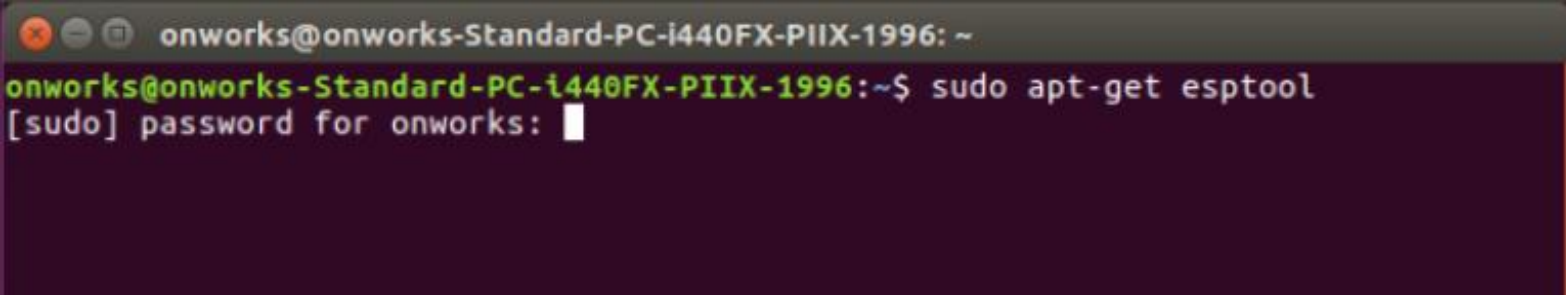
\includegraphics[width=1\textwidth]{figures/apt_get_esptool.png}
    \caption{Installation du paquet esptool sous Ubuntu.}
\end{figure}

Ensuite, vous devez installer Python si vous ne l'avez pas déjà, car l'outil esptool est écrit en langage Python.
Vous devez donc taper la commande \textit{“sudo apt-get python”}, comme le montre l'image. À nouveau, si vous y êtes
invité, saisissez le mot de passe de l'utilisateur sudo, appuyez sur ENTREE et patientez.

\begin{figure}[H]
    \centering
    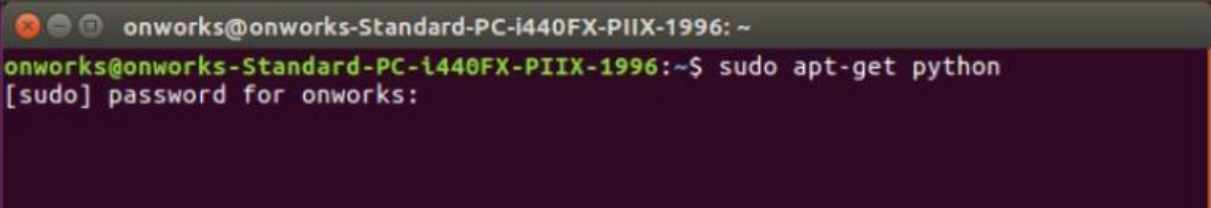
\includegraphics[width=1\textwidth]{figures/apt_get_python.png}
    \caption{Installation du paquet python sous Ubuntu.}
\end{figure}

Une fois les deux paquets installés, tapez \textit{“sudo tail -f /var/log/messages”} dans le
terminal comme indiqué sur l'image pour surveiller en temps réel le fichier journal (log) qui nous indiquera
à quel port COM le boîtier noir sera associé par le système d'exploitation.~Si vous y êtes invité, saisissez le
mot de passe de l'utilisateur sudo, puis appuyez sur ENTREE.~\textbf{Nous pouvons maintenant brancher le boîtier noir}.

\begin{figure}[H]
    \centering
    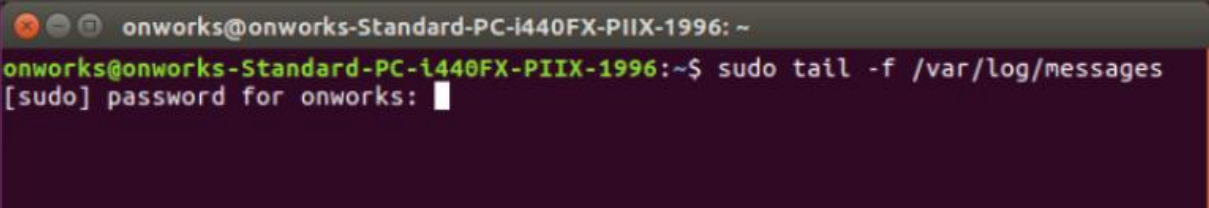
\includegraphics[width=1\textwidth]{figures/tail_com.png}
    \caption{Surveillance en temps réel des connexions COM.}
\end{figure}

Le boîtier noir possède un petit connecteur microUSB sur sa face arrière, comme vous pouvez le voir
sur la Figure~\ref{fig:black_box_labels}. Connectez donc l'extrémité du câble microUSB au
boîtier noir. Ensuite, connectez l'extrémité USB du câble à un port USB libre de votre ordinateur.

\textbf{RAPPEL !} Les deux côtés du câble ne s'insèrent que dans un seul sens dans leurs prises respectives,
ne forcez donc pas au risque de casser le port du ToM+ ou celui de votre ordinateur. Essayez de le tourner
de l'autre côté et vérifiez si cela fonctionne ainsi.\\

Dès que vous branchez le boîtier noir à l'ordinateur, vous devriez obtenir une sortie similaire
à celle présentée dans le bloc de code ci-dessous.

\begin{lstlisting}[language=bash]
Oct 15 11:05:14 Kubuntu2004 kernel: [ 172.232228] usb 1-3: new full-speed USB
device number 3 using xhci_hcd
Oct 15 11:05:14 Kubuntu2004 kernel: [ 172.423441] usb 1-3: New USB device found,
idVendor=10c4, idProduct=ea60, bcdDevice= 1.00
Oct 15 11:05:14 Kubuntu2004 kernel: [ 172.423453] usb 1-3: New USB device
strings: Mfr=1, Product=2, SerialNumber=3
Oct 15 11:05:14 Kubuntu2004 kernel: [ 172.423457] usb 1-3: Product: CP2102 USB
to UART Bridge Controller
Oct 15 11:05:14 Kubuntu2004 kernel: [ 172.423461] usb 1-3: Manufacturer: Silicon
Labs
85
Oct 15 11:05:14 Kubuntu2004 kernel: [ 172.423464] usb 1-3: SerialNumber: 0001
Oct 15 11:05:14 Kubuntu2004 mtp-probe: checking bus 1, device 3:
"/sys/devices/pci0000:00/0000:00:08.1/0000:03:00.3/usb1/1-3"
Oct 15 11:05:14 Kubuntu2004 mtp-probe: bus: 1, device: 3 was not an MTP device
Oct 15 11:05:14 Kubuntu2004 kernel: [ 172.457397] usbcore: registered new
interface driver usbserial_generic
Oct 15 11:05:14 Kubuntu2004 kernel: [ 172.457415] usbserial: USB Serial support
registered for generic
Oct 15 11:05:14 Kubuntu2004 kernel: [ 172.460166] usbcore: registered new
interface driver cp210x
Oct 15 11:05:14 Kubuntu2004 kernel: [ 172.460185] usbserial: USB Serial support
registered for cp210x
Oct 15 11:05:14 Kubuntu2004 kernel: [ 172.460236] cp210x 1-3:1.0: cp210x
converter detected
Oct 15 11:05:14 Kubuntu2004 kernel: [ 172.464538] usb 1-3: cp210x converter now
attached to ttyUSB0
Oct 15 11:05:14 Kubuntu2004 mtp-probe: checking bus 1, device 3:
"/sys/devices/pci0000:00/0000:00:08.1/0000:03:00.3/usb1/1-3"
Oct 15 11:05:14 Kubuntu2004 mtp-probe: bus: 1, device: 3 was not an MTP device
\end{lstlisting}

La ligne qui nous intéresse particulièrement est la suivante : \textit{“cp210x converter now
attached to ttyUSB0”} où le terme \textbf{“ttyUSB0”} correspond au port
série auquel le boîtier noir est connecté. Notez ce nom de port (qui peut différer du mien), car nous en
aurez besoin pour téléverser le nouveau firmware.

\subsection{Déroulement de la mise à jour}

Naviguez avec votre gestionnaire de fichiers dans le dossier où se trouve le fichier \textit{.bin} du firmware,
puis ouvrez un terminal à cet endroit en faisant un clic droit sur le dossier et en choisissant l'option \textbf{“Ouvrir dans un terminal”}
dans le menu déroulant. Si vous préférez, vous pouvez naviguer manuellement à travers vos dossiers
à l'aide de la commande « cd » jusqu'à trouver le bon répertoire.

Une fois dans le bon dossier, exécutez cette commande longue et un peu fastidieuse, en remplaçant \textit{“ttyUSBx”} par le
nom du port série noté précédemment (ex. \textit{“ttyUSB0”}) et \textit{“ESP32\textunderscore FwXX.bin”} par
le nom du fichier \textit{“.bin”} qui contient la version du firmware à charger sur le ToM+
(ex. \textit{“ESP32\textunderscore Fw23.bin”}).

\begin{verbatim}
    python /usr/share/esptool/esptool.py --chip auto --port /dev/ttyUSBx --baud
921600 --before default_reset --after hard_reset write_flash -z --flash_mode dio
--flash_freq 40m --flash_size 4MB 0x10000 ESP32_FwXX.bin
\end{verbatim}

Vous devriez obtenir une sortie similaire à la suivante :

\begin{lstlisting}[language=bash]
Serial port /dev/ttyUSB0
Connecting........_____.....____
Detecting chip type... ESP32
Chip is ESP32D0WDQ5 (revision 3)
Features: WiFi, BT, Dual Core, 240MHz, VRef calibration in efuse, Coding Scheme
None
Crystal is 40MHz
MAC: xx:xx:xx:xx:xx:xx
Changing baud rate to 921600
Changed.
Enabling default SPI flash mode...
Configuring flash size...
Erasing flash...
Compressed 716176 bytes to 461048...
Took 2.90s to erase flash block
Wrote 716176 bytes (461048 compressed) at 0x00010000 in 9.1 seconds (effective
630.3 kbit/s)...
Hash of data verified.
Leaving...
Hard resetting via RTS pin...
\end{lstlisting}

Fermez cette fenêtre ainsi que toutes les autres, puis débranchez le câble en toute sécurité
du PC et du ToM+. Ce n'est qu'après ces actions que vous pourrez rétablir l'alimentation normale du ToM+,
en basculant l'interrupteur sur la position 1 et en mettant le contact de votre Twizy avec la clé.

Pour restaurer vos configurations précédentes, accédez à la page des paramètres du ToM+ en appuyant sur
les trois points dans le coin supérieur droit, puis appuyez sur le bouton de sortie sans rien
modifier. De cette façon, vous mettrez à jour la structure des données enregistrées dans la mémoire
du boîtier noir et vos configurations seront à nouveau opérationnelles.\\

\textbf{Félicitations !} Vous avez terminé l'ensemble de la procédure de mise à jour. Profitez bien du nouveau firmware,
et n'oubliez pas de me signaler tout bug ou problème par message privé, idéalement en joignant une photo.
